%********************************************************************
% Kapitel 5: Implementierung
%********************************************************************
\chapter{Implementierung}
\label{ch:implementierung}

Dieses Kapitel beschreibt die Implementierung des konzipierten Netzwerk-Monitoring-Systems. Ziel der Implementierung ist es, die in Kapitel~\ref{ch:konzeption} beschriebenen Lösungsansätze als funktionsfähigen Proof-of-Concept umzusetzen. Dabei werden die wesentlichen Umsetzungstechnologien, die Struktur der Anwendung, die periodische Prüfung von Netzwerkzielen, die Bereitstellung von Metriken, die REST-Schnittstellen, das Incident-Management sowie die containerisierte Ausführung erläutert.

Es werden ausschließlich ausgewählte Implementierungsdetails dargestellt. Eine vollständige Wiedergabe des Quellcodes ist nicht Ziel dieses Kapitels. Stattdessen werden diejenigen Komponenten und Abläufe betrachtet, die für die technische Umsetzung der Anforderungen und die Nachvollziehbarkeit der Lösung wesentlich sind.

\section{Umsetzungstechnologien}
\label{sec:umsetzungstechnologien}

Für die Umsetzung wurde eine Java-basierte Anwendung gewählt. Das Projekt ist als Maven-Projekt aufgebaut und verwendet eine modulare Paketstruktur. Die aktuelle Implementierung enthält unter anderem die Pakete \texttt{config}, \texttt{controller}, \texttt{model}, \texttt{service}, \texttt{scheduler}, \texttt{alert} und \texttt{incident}. Dadurch werden technische Aufgaben und fachliche Verantwortlichkeiten voneinander getrennt \cite{projekt-repository}.

\subsection{Java und Spring Boot}
\label{subsec:java-spring-boot}

Java wurde als Programmiersprache gewählt, da die Sprache eine ausgereifte Unterstützung für Netzwerkkommunikation, Nebenläufigkeit, Datenbankzugriffe und serverseitige Anwendungen bietet. Zusätzlich erleichtert die statische Typisierung die Wartbarkeit und Nachvollziehbarkeit der Implementierung.

Spring Boot wurde als Anwendungsrahmen eingesetzt. Die Wahl begründet sich insbesondere durch die vorhandene Unterstützung für:

\begin{itemize}
    \item REST-basierte HTTP-Schnittstellen,
    \item externe Anwendungskonfiguration,
    \item Dependency Injection,
    \item geplante beziehungsweise periodische Aufgaben,
    \item Sicherheitskonfiguration,
    \item Datenbankzugriffe und Persistenz,
    \item Integration von Monitoring- und Metrikfunktionen.
\end{itemize}

Die Anwendung wird über eine zentrale Startklasse gestartet. Die fachliche Logik ist dabei nicht in der Startklasse konzentriert, sondern auf mehrere Komponenten verteilt.

\subsection{Maven}
\label{subsec:maven}

Maven übernimmt die Verwaltung der Abhängigkeiten, den Build-Prozess und die Erstellung des ausführbaren Artefakts. Die verwendeten Bibliotheken und Plugins werden in der Datei \texttt{pom.xml} definiert.

Durch die deklarative Abhängigkeitsverwaltung kann der Build-Prozess reproduzierbar ausgeführt werden. Dies ist insbesondere für die spätere containerisierte Bereitstellung relevant, da das Docker-Image auf einem definierten Build-Ergebnis basiert.

\subsection{Persistenz}
\label{subsec:persistenz-technologie}

Für die Persistierung der Prüfergebnisse und Incidents wird eine relationale Datenbank verwendet. Die Datenbank speichert unter anderem:

\begin{itemize}
    \item konfigurierte Netzwerkziele,
    \item durchgeführte Prüfungen,
    \item Status- und Latenzwerte,
    \item Alert-Informationen,
    \item den Status eines Incidents,
    \item Erstellungs- und Auflösungszeitpunkte.
\end{itemize}

Die Entscheidung für eine relationale Persistenzlösung wurde getroffen, weil Prüfergebnisse und Incidents klar strukturierte Attribute besitzen und über Zeitpunkte, Statuswerte sowie Zielsysteme abgefragt werden können.

\subsection{Docker und Docker Compose}
\label{subsec:docker-compose-implementierung}

Die Anwendung wird in einem Docker-Container ausgeführt. Die Datei \texttt{Dockerfile} beschreibt den Aufbau des Anwendungsimages. Die weiteren Monitoring-Komponenten werden über eine Docker-Compose-Konfiguration gestartet.

Die containerisierte Bereitstellung bietet folgende Vorteile:

\begin{itemize}
    \item reproduzierbare Umgebung,
    \item einheitlicher Start der beteiligten Komponenten,
    \item Trennung der Anwendung von der lokalen Host-Umgebung,
    \item einfache Weitergabe des Proof-of-Concept,
    \item zentrale Definition von Netzwerken, Ports und Volumes.
\end{itemize}

Die Wahl von Docker Compose ist insbesondere für die lokale Entwicklung, Demonstration und Evaluation geeignet, da mehrere voneinander abhängige Services gemeinsam verwaltet werden können \cite{docker-compose-documentation}.

\section{Anwendungsstruktur}
\label{sec:anwendungsstruktur}

Die Anwendung ist nach fachlichen und technischen Verantwortlichkeiten strukturiert. Abbildung~\ref{fig:implementierungsstruktur} stellt die wesentlichen Module der Implementierung dar.

\begin{figure}[htbp]
    \centering
    % TODO: Eigene Abbildung der Paket- beziehungsweise Modulstruktur einfügen.
    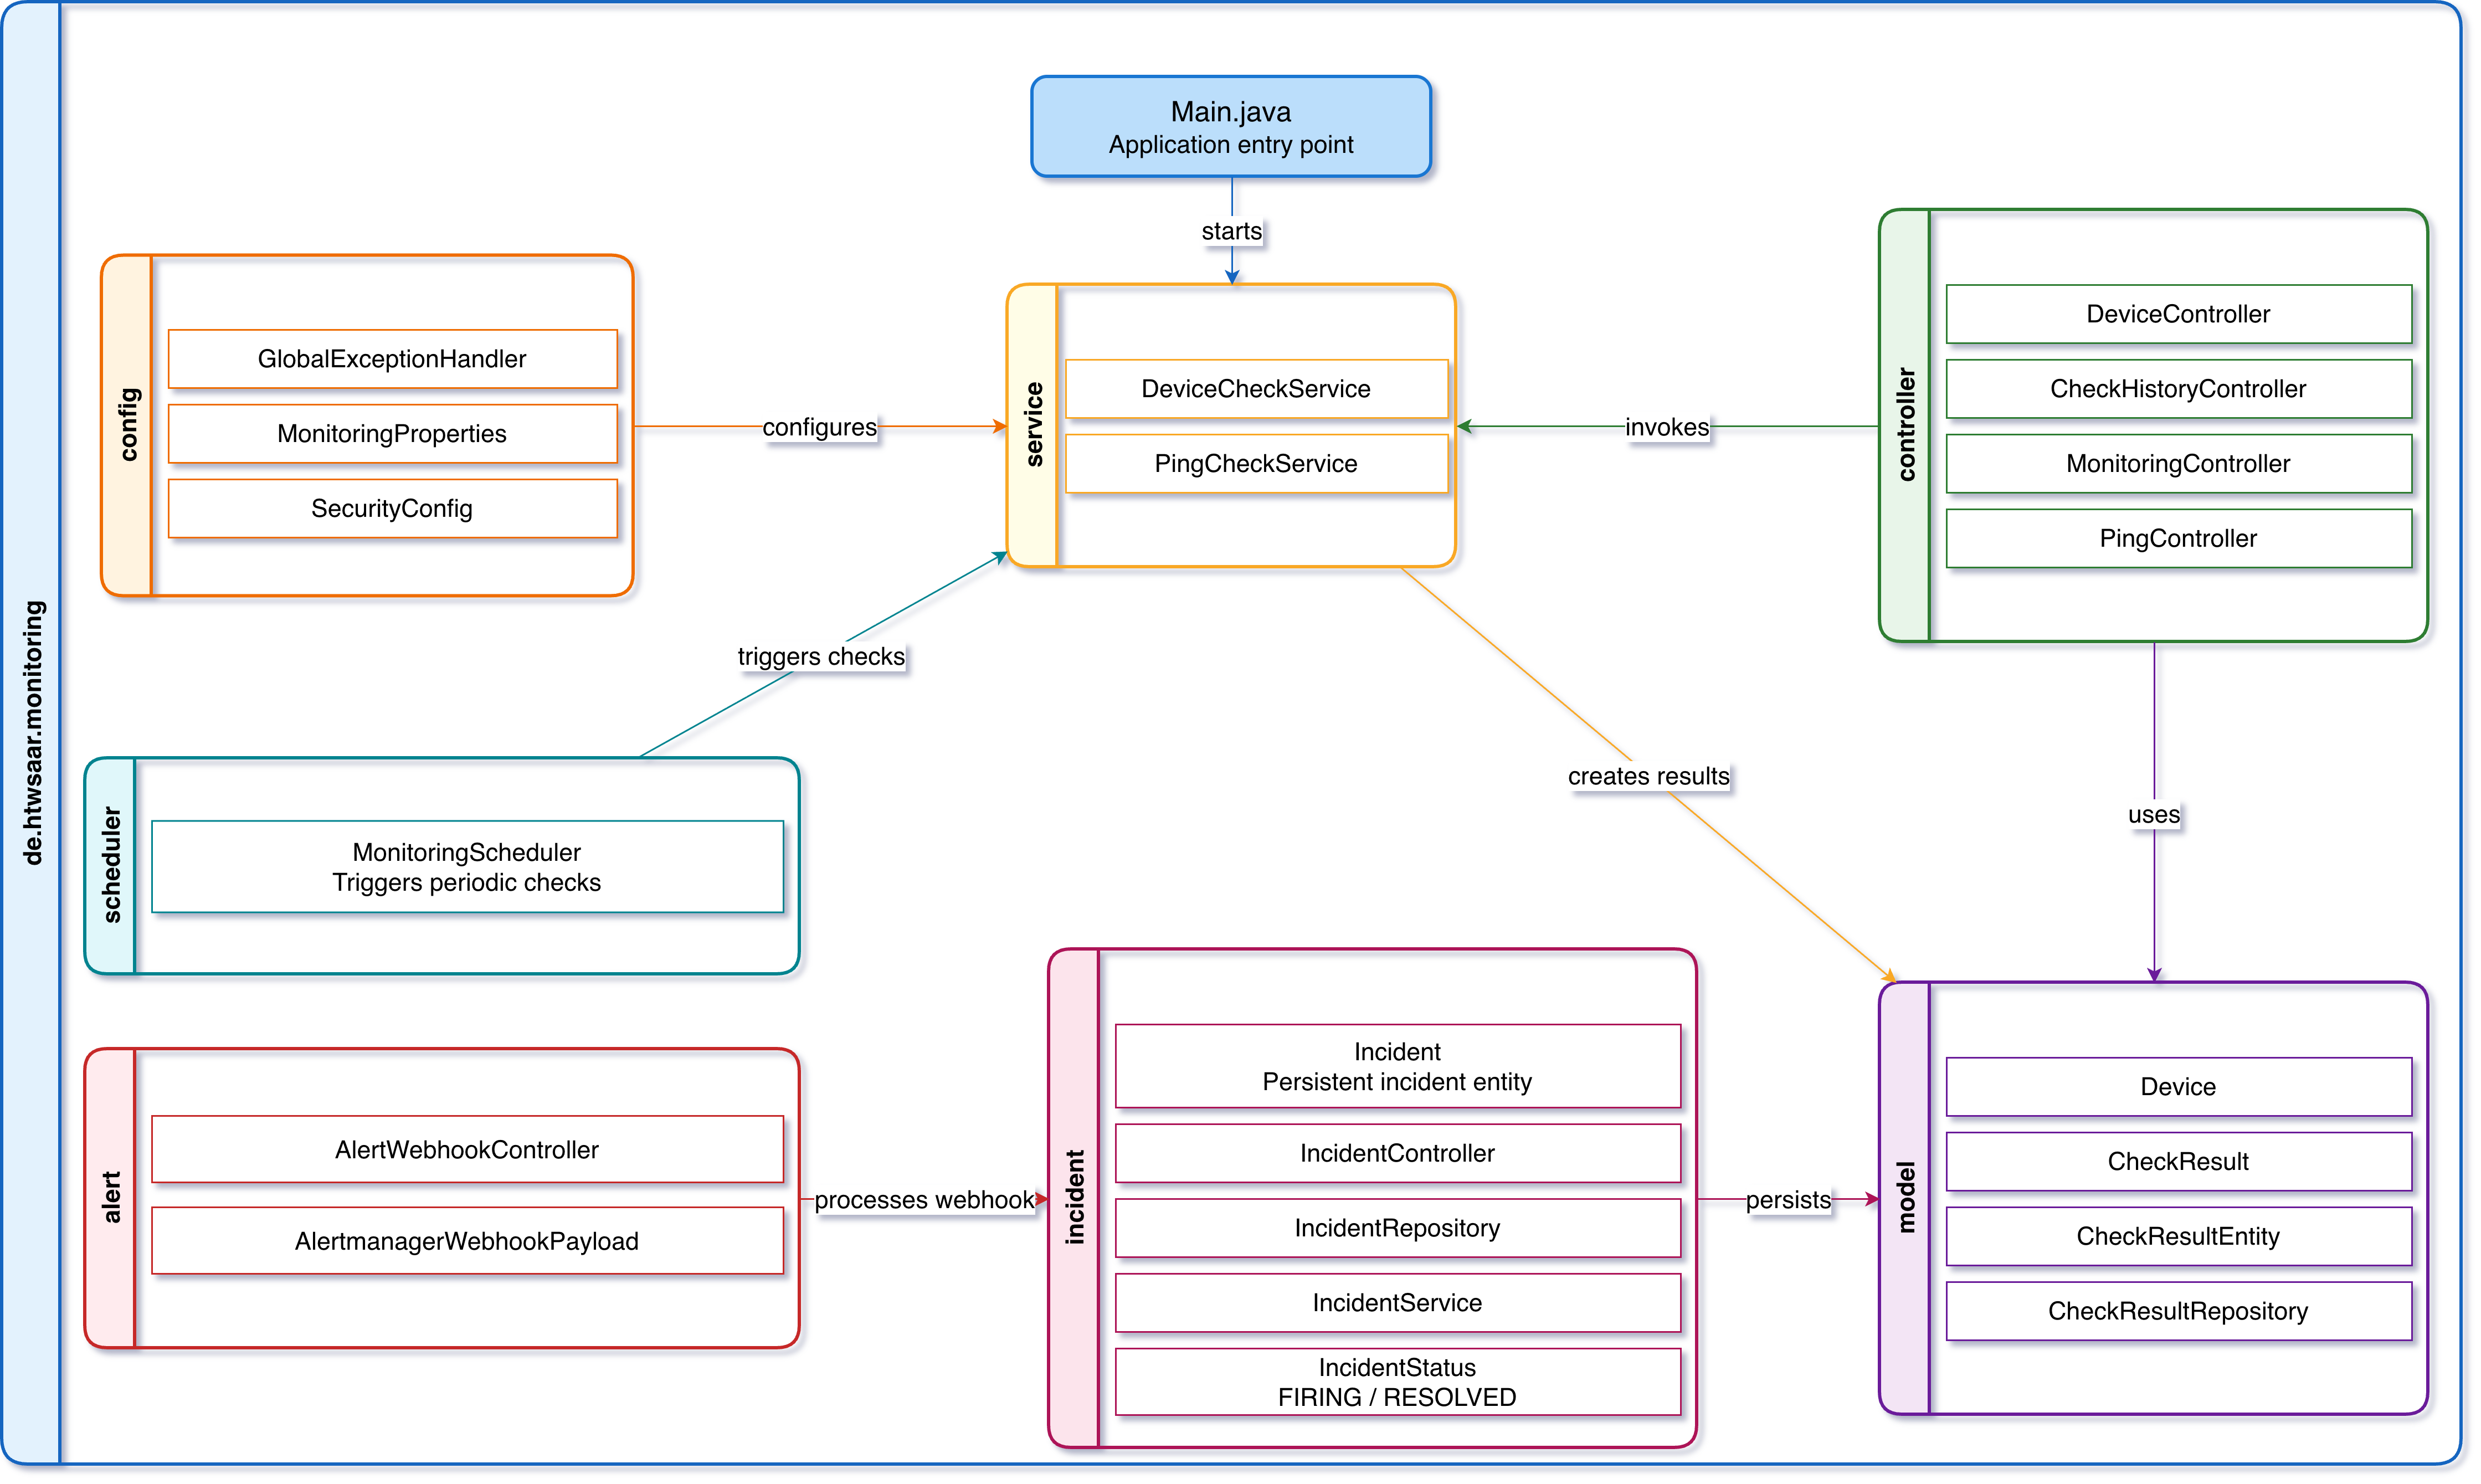
\includegraphics[width=1.0\textwidth]{Chapters/Graphics/Implementierungsstruktur.drawio.png}
    \caption{Struktur der implementierten Anwendung}
    \label{fig:implementierungsstruktur}
\end{figure}

Die wichtigsten Pakete und ihre Aufgaben sind:

\begin{description}
    \item[\texttt{config}:] Zentrale Konfiguration, Sicherheit und globale Fehlerbehandlung.
    \item[\texttt{controller}:] REST-Schnittstellen für Geräte, Prüfhistorie, Monitoring und manuelle Prüfungen.
    \item[\texttt{model}:] Domänenobjekte und Persistenzmodelle für Geräte und Prüfergebnisse.
    \item[\texttt{service}:] Fachliche Logik für Geräteprüfungen und Erreichbarkeitsmessungen.
    \item[\texttt{scheduler}:] Zeitgesteuerte Ausführung der regelmäßigen Prüfzyklen.
    \item[\texttt{alert}:] Verarbeitung von Alert-Webhooks und Abbildung eingehender Alert-Daten.
    \item[\texttt{incident}:] Verwaltung, Speicherung und Abfrage von Incidents.
\end{description}

Die Struktur unterstützt das Prinzip der Trennung von Verantwortlichkeiten. Controller nehmen Anfragen entgegen, Services führen fachliche Verarbeitung durch und Repository-Komponenten übernehmen den Datenzugriff.

\section{Konfiguration der Überwachungsziele}
\label{sec:konfiguration-ueberwachungsziele}

Die Überwachungsparameter werden nicht fest in der Prüflogik programmiert, sondern über die Anwendungskonfiguration bereitgestellt. Die Klasse \texttt{MonitoringProperties} bündelt die relevanten Konfigurationswerte.

Zu den konfigurierbaren Informationen gehören insbesondere:

\begin{itemize}
    \item Name eines Überwachungsziels,
    \item Hostname oder IP-Adresse,
    \item zu prüfender Port,
    \item Aktivierungsstatus,
    \item Prüfintervall,
    \item Verbindungs- beziehungsweise Prüf-Timeout.
\end{itemize}

Ein vereinfachtes Beispiel der Konfiguration ist in Listing~\ref{lst:monitoring-konfiguration} dargestellt.

\begin{lstlisting}[
    language={},
    caption={Beispielhafte Konfiguration eines Überwachungsziels},
    label={lst:monitoring-konfiguration}
]
monitoring:
  interval: 10000
  timeout: 2000
  devices:
    - name: router
      host: 192.0.2.1
      port: 443
      enabled: true
\end{lstlisting}

Die konkreten Schlüssel und Werte müssen an die tatsächlich verwendete \texttt{application.yml} angepasst werden. Entscheidend ist die technische Trennung zwischen Konfiguration und Prüflogik. Dadurch können Überwachungsziele verändert werden, ohne die Java-Klassen neu implementieren zu müssen.

Zusätzliche umgebungsabhängige Werte werden über Umgebungsvariablen beziehungsweise eine Beispieldatei für Umgebungsvariablen bereitgestellt. Sensible Werte werden dadurch nicht zwingend direkt in den Quellcode aufgenommen.

\section{Implementierung der Geräteprüfung}
\label{sec:implementierung-geraetepruefung}

Die zentrale fachliche Funktion ist die Prüfung eines konfigurierten Netzwerkziels. Die Implementierung ist in den Service-Komponenten der Anwendung gekapselt.

\subsection{Prüfung der Erreichbarkeit}
\label{subsec:pruefung-erreichbarkeit}

Für jedes aktivierte Gerät wird eine Verbindung zu der konfigurierten Kombination aus Host und Port aufgebaut. Vor Beginn der Prüfung wird ein Zeitstempel erfasst. Nach Abschluss der Verbindung wird aus der Differenz zwischen Start- und Endzeitpunkt die Dauer des Verbindungsversuchs berechnet.

Der grundsätzliche Ablauf ist:

\begin{enumerate}
    \item Laden der aktivierten Überwachungsziele.
    \item Erfassung des Startzeitpunkts.
    \item Aufbau einer TCP-Verbindung zu Host und Port.
    \item Anwendung des konfigurierten Timeouts.
    \item Ermittlung des Erreichbarkeitsstatus.
    \item Berechnung der Latenz bei erfolgreicher Verbindung.
    \item Erfassung einer Fehlermeldung bei einem fehlgeschlagenen Versuch.
    \item Speicherung und Veröffentlichung des Prüfergebnisses.
\end{enumerate}

Ein vereinfachter Ausschnitt des Ablaufs ist in Listing~\ref{lst:prueflogik} dargestellt.

\begin{lstlisting}[
    language=Java,
    caption={Vereinfachter Ablauf einer Geräteprüfung},
    label={lst:prueflogik}
]
long start = System.nanoTime();

try {
    // Verbindung zu Host und Port mit Timeout herstellen
    boolean reachable = checkConnection(device);

    long duration = System.nanoTime() - start;
    long latencyMs = duration / 1_000_000;

    saveResult(device, reachable, latencyMs, null);
} catch (Exception exception) {
    long duration = System.nanoTime() - start;
    long latencyMs = duration / 1_000_000;

    saveResult(device, false, latencyMs, exception.getMessage());
}
\end{lstlisting}

Der dargestellte Code ist bewusst verkürzt und dient ausschließlich der Erläuterung des Prinzips. Die konkrete Implementierung enthält zusätzliche Verarbeitungsschritte für Persistenz, Metrikaktualisierung und Fehlerbehandlung.

\subsection{Fehlerbehandlung}
\label{subsec:implementierung-fehlerbehandlung}

Ein einzelnes nicht erreichbares Ziel darf den Prüfzyklus der übrigen Ziele nicht beenden. Deshalb wird die Prüfung pro Ziel isoliert behandelt. Netzwerkfehler und Timeouts werden als fehlgeschlagene Prüfergebnisse erfasst.

Mögliche Fehlerfälle sind:

\begin{itemize}
    \item Verbindungs-Timeout,
    \item verweigerte Verbindung,
    \item nicht auflösbarer Hostname,
    \item ungültige Konfiguration,
    \item unerwartete Ausnahme während des Verbindungsaufbaus.
\end{itemize}

Die Klasse \texttt{GlobalExceptionHandler} übernimmt zusätzlich die zentrale Behandlung von Fehlern, die während der Verarbeitung von HTTP-Anfragen auftreten. Dadurch können Fehlerantworten einheitlich an API-Clients zurückgegeben werden.

\section{Zeitgesteuerte Ausführung}
\label{sec:zeitgesteuerte-ausfuehrung}

Die regelmäßige Ausführung der Geräteprüfungen wird durch die Klasse \texttt{MonitoringScheduler} realisiert. Der Scheduler startet in dem konfigurierten Intervall einen Prüfzyklus.

Abbildung~\ref{fig:pruefzyklus-implementierung} zeigt den vereinfachten Ablauf.

\begin{figure}[htbp]
    \centering
    % TODO: Ablaufdiagramm des implementierten Prüfzyklus einfügen.
    % \includegraphics[width=0.75\textwidth]{Graphics/implementierter-pruefzyklus.pdf}
    \caption{Implementierter Ablauf eines periodischen Prüfzyklus}
    \label{fig:pruefzyklus-implementierung}
\end{figure}

Die Ablaufkette besteht aus:

\begin{enumerate}
    \item Scheduler erhält ein zeitgesteuertes Ausführungssignal.
    \item Der Prüfservice lädt die konfigurierten Ziele.
    \item Nicht aktivierte Ziele werden übersprungen.
    \item Aktivierte Ziele werden einzeln geprüft.
    \item Die Ergebnisse werden gespeichert und als aktuelle Zustände bereitgestellt.
\end{enumerate}

Zusätzlich existiert eine Möglichkeit, einen Prüfzyklus über einen REST-Endpunkt manuell auszulösen. Diese Funktion ist für Tests, Demonstrationen und die Fehlersuche relevant.

\section{Modellierung und Persistierung}
\label{sec:modellierung-persistierung}

Die Modellklassen bilden die fachlichen Objekte des Systems ab. Im aktuellen Projekt existieren unter anderem Klassen für Geräte, Prüfergebnisse und deren persistierte Repräsentationen.

\subsection{Gerätemodell}
\label{subsec:geraetemodell}

Das Gerätemodell enthält die Informationen, die für eine Erreichbarkeitsprüfung erforderlich sind. Dazu gehören mindestens:

\begin{itemize}
    \item eine eindeutige Identifikation,
    \item ein Anzeigename,
    \item Hostname oder IP-Adresse,
    \item Portnummer,
    \item Aktivierungsstatus.
\end{itemize}

Die Trennung zwischen Gerätemodell und Prüfresultat ermöglicht es, eine Gerätekonfiguration unabhängig von einzelnen Messungen zu verwalten.

\subsection{Prüfergebnis}
\label{subsec:pruefergebnis}

Ein Prüfergebnis beschreibt den Zustand eines Geräts zu einem bestimmten Zeitpunkt. Es umfasst:

\begin{itemize}
    \item das geprüfte Gerät,
    \item den Erreichbarkeitsstatus,
    \item die gemessene Latenz,
    \item den Prüfzeitpunkt,
    \item eine optionale Fehlermeldung.
\end{itemize}

Für die langfristige Speicherung wird das Ergebnis in einer persistierbaren Entität abgebildet. Ein Repository ermöglicht den Zugriff auf aktuelle und historische Ergebnisse.

\begin{lstlisting}[
    language=Java,
    caption={Vereinfachtes Modell eines Prüfergebnisses},
    label={lst:checkresult-modell}
]
public class CheckResult {
    private String deviceName;
    private boolean reachable;
    private long latencyMs;
    private Instant timestamp;
    private String errorMessage;
}
\end{lstlisting}

Der Code ist exemplarisch verkürzt. Die konkrete Implementierung kann zusätzliche Konstruktoren, Zugriffsmethoden, Validierungen oder Persistenzannotationen enthalten.

\section{Implementierung der REST-Schnittstellen}
\label{sec:implementierung-rest}

Die REST-Schnittstellen sind in mehreren Controller-Klassen organisiert. Diese Aufteilung verhindert, dass eine einzelne Controller-Klasse sämtliche Funktionen des Systems enthält.

\subsection{Geräte- und Monitoring-Schnittstellen}
\label{subsec:geraete-monitoring-api}

Der \texttt{DeviceController} stellt Funktionen für die Abfrage der konfigurierten Geräte bereit. Der \texttt{MonitoringController} übernimmt allgemeine Monitoring-Funktionen, beispielsweise die Abfrage des Dienststatus oder die manuelle Auslösung eines Prüfzyklus.

Der \texttt{CheckHistoryController} stellt historische Prüfergebnisse bereit. Dadurch kann ein Client aktuelle Zustände und vergangene Messwerte getrennt abfragen.

Ein vereinfachtes Beispiel eines REST-Endpunkts ist in Listing~\ref{lst:rest-endpunkt} dargestellt.

\begin{lstlisting}[
    language=Java,
    caption={Vereinfachter REST-Endpunkt zur Abfrage der Prüfhistorie},
    label={lst:rest-endpunkt}
]
@GetMapping("/history")
public List<CheckResult> getHistory() {
    return checkHistoryService.findAll();
}
\end{lstlisting}

Die konkrete URL-Struktur und die Rückgabetypen müssen an die tatsächlich implementierten Controller angepasst werden.

\subsection{Manuelle Prüfungen}
\label{subsec:manuelle-pruefungen}

Für Test- und Diagnosezwecke kann ein Prüfzyklus manuell über eine HTTP-Anfrage ausgelöst werden. Dadurch kann geprüft werden, ob Änderungen an der Konfiguration oder am Zielsystem unmittelbar erkannt werden.

Die manuelle Auslösung ist insbesondere für den Proof-of-Concept wichtig, da sie eine reproduzierbare Demonstration einzelner Systemzustände ermöglicht.

\subsection{Sicherheit der API}
\label{subsec:api-sicherheit-implementierung}

Die Klasse \texttt{SecurityConfig} enthält die Sicherheitskonfiguration der Anwendung. Administrative oder verändernde Endpunkte werden gegenüber rein lesenden Endpunkten unterschieden.

Die Sicherheitskonfiguration verfolgt insbesondere folgende Ziele:

\begin{itemize}
    \item Schutz administrativer Funktionen,
    \item Vermeidung unautorisierter manueller Prüfungen,
    \item zentrale Definition der Zugriffsregeln,
    \item externe Bereitstellung sensibler Konfigurationswerte.
\end{itemize}

Die tatsächliche Absicherung der einzelnen Endpunkte sollte in der Dokumentation exakt entsprechend der implementierten Security-Konfiguration beschrieben werden.

\section{Metriken und Monitoring-Integration}
\label{sec:metriken-monitoring-integration}

Die Implementierung stellt die Ergebnisse der Geräteprüfungen als Monitoring-Daten bereit. Für jedes Gerät werden mindestens der Erreichbarkeitsstatus und die Latenz berücksichtigt.

Ein vereinfachtes Metrikmodell ist:

\begin{itemize}
    \item \texttt{network\_device\_up}: Wert 1 für erreichbar und 0 für nicht erreichbar.
    \item \texttt{network\_device\_latency\_ms}: Dauer des letzten Verbindungsversuchs in Millisekunden.
\end{itemize}

Die Geräte werden über Labels oder vergleichbare Merkmale unterschieden. Dadurch können einzelne Geräte in Abfragen und Dashboards separat dargestellt werden.

\begin{lstlisting}[
    caption={Beispielhafte Darstellung exportierter Monitoring-Metriken},
    label={lst:metrics-export}
]
# HELP network_device_up Current availability status
# TYPE network_device_up gauge
network_device_up{device="router"} 1

# HELP network_device_latency_ms Last connection latency
# TYPE network_device_latency_ms gauge
network_device_latency_ms{device="router"} 12
\end{lstlisting}

Die konkrete Benennung der Metriken und Labels muss mit dem tatsächlichen Export der Anwendung übereinstimmen. Für die technische Integration werden die im Projekt konfigurierten Monitoring-Komponenten verwendet.

\section{Alert-Webhooks und Incident-Management}
\label{sec:alert-incident-implementierung}

Die Alert-Verarbeitung ist in einem eigenen Paket organisiert. Der \texttt{AlertWebhookController} empfängt eingehende Alert-Nachrichten. Das Datenmodell \texttt{AlertmanagerWebhookPayload} bildet die Struktur des empfangenen Webhook-Inhalts ab.

\subsection{Verarbeitung eingehender Alerts}
\label{subsec:alert-verarbeitung}

Beim Empfang eines Alerts werden die relevanten Informationen aus dem Payload extrahiert. Dazu zählen beispielsweise:

\begin{itemize}
    \item Alert-Name,
    \item Status des Alerts,
    \item Labels,
    \item Annotations,
    \item betroffener Überwachungsdienst oder Zielname,
    \item Startzeitpunkt,
    \item optionaler Auflösungszeitpunkt.
\end{itemize}

Anschließend wird der Alert an den \texttt{IncidentService} weitergeleitet. Die Zuständigkeit für die Geschäftslogik bleibt somit im Service und wird nicht direkt im Controller implementiert.

\subsection{Incident-Modell}
\label{subsec:incident-modell-implementierung}

Das Incident-Modell wird durch die Klasse \texttt{Incident} repräsentiert. Der Status wird über das Enum \texttt{IncidentStatus} modelliert. Dadurch sind nur definierte Zustände wie beispielsweise \texttt{FIRING} und \texttt{RESOLVED} zulässig.

Das Repository stellt den Datenzugriff bereit. Der \texttt{IncidentService} implementiert die fachliche Verarbeitung, insbesondere:

\begin{itemize}
    \item Erstellen eines neuen Incidents,
    \item Erkennen bereits vorhandener aktiver Incidents,
    \item Aktualisieren eines bestehenden Incidents,
    \item Verarbeitung eines aufgelösten Alerts,
    \item Abfrage aktiver und historischer Incidents.
\end{itemize}

Durch die Verwendung eines Alert-Fingerprints oder einer vergleichbaren Identifikation kann verhindert werden, dass derselbe aktive Alert bei wiederholter Zustellung mehrfach als neues Incident gespeichert wird.

\subsection{REST-Abfrage der Incidents}
\label{subsec:incident-api-implementierung}

Der \texttt{IncidentController} stellt die Incident-Historie für externe Clients bereit. Typische Abfragen sind:

\begin{itemize}
    \item alle Incidents,
    \item aktive Incidents,
    \item ein einzelnes Incident,
    \item Incidents nach Status oder Zeitraum.
\end{itemize}

Die Incident-Historie ergänzt die Zeitreihendaten um eine fachlich interpretierbare Darstellung von Störungen.

\section{Globale Fehlerbehandlung}
\label{sec:globale-fehlerbehandlung}

Die Klasse \texttt{GlobalExceptionHandler} bündelt die Behandlung ausgewählter Fehler, die während der Verarbeitung von REST-Anfragen auftreten. Ohne eine zentrale Fehlerbehandlung könnten unterschiedliche Controller inkonsistente Antwortformate liefern.

Eine einheitliche Fehlerantwort kann beispielsweise folgende Informationen enthalten:

\begin{itemize}
    \item HTTP-Statuscode,
    \item Zeitpunkt des Fehlers,
    \item Fehlernachricht,
    \item betroffener Request-Pfad.
\end{itemize}

Die zentrale Behandlung verbessert die Wartbarkeit der API und erleichtert die Diagnose während des Betriebs.

\section{Containerisierte Bereitstellung}
\label{sec:containerisierte-bereitstellung-implementierung}

Die Anwendung wird über ein Dockerfile in ein Container-Image überführt. Der Build-Prozess umfasst typischerweise:

\begin{enumerate}
    \item Bereitstellung einer geeigneten Java-Laufzeitumgebung.
    \item Kopieren des erzeugten Anwendungspakets in das Image.
    \item Festlegen des Startbefehls.
    \item Öffnen beziehungsweise Dokumentieren des Anwendungsports.
\end{enumerate}

Die Datei \texttt{docker-compose.yml} beschreibt die gemeinsame Ausführung der Anwendung und der unterstützenden Monitoring-Komponenten.

Ein vereinfachter Ausschnitt ist in Listing~\ref{lst:docker-compose} dargestellt.

\begin{lstlisting}[
    language={},
    caption={Vereinfachtes Beispiel der containerisierten Bereitstellung},
    label={lst:docker-compose}
]
services:
  monitoring:
    build: .
    ports:
      - "8080:8080"

  prometheus:
    image: prom/prometheus

  grafana:
    image: grafana/grafana
\end{lstlisting}

Der tatsächliche Compose-Ausschnitt muss entsprechend der aktuellen Projektdatei angepasst werden. Insbesondere Namen, Ports, Volumes, Netzwerke und Umgebungsvariablen dürfen in der finalen Arbeit nicht abweichend vom Repository dargestellt werden.

\subsection{Persistente Daten}
\label{subsec:persistente-daten-container}

Daten, die den Neustart eines Containers überleben müssen, werden über Volumes oder gemountete Verzeichnisse gespeichert. Dies betrifft insbesondere:

\begin{itemize}
    \item Zeitreihendaten,
    \item Incident-Daten,
    \item Grafana-Konfiguration,
    \item Monitoring-Konfigurationen.
\end{itemize}

Damit wird verhindert, dass bei jedem Neustart der Container sämtliche historischen Daten verloren gehen.

\section{Proof-of-Concept}
\label{sec:proof-of-concept}

Die Implementierung stellt einen funktionsfähigen Proof-of-Concept dar. Die wesentlichen Kernfunktionen aus der Konzeption sind technisch umgesetzt:

\begin{itemize}
    \item konfigurierbare Überwachungsziele,
    \item periodische Netzwerkprüfungen,
    \item Speicherung von Prüfergebnissen,
    \item Bereitstellung einer REST-Schnittstelle,
    \item Bereitstellung von Monitoring-Metriken,
    \item Empfang von Alert-Webhooks,
    \item Verwaltung einer Incident-Historie,
    \item containerisierte Ausführung.
\end{itemize}

Der Proof-of-Concept erhebt nicht den Anspruch, sämtliche Anforderungen eines vollständigen Enterprise-Monitoring-Systems abzudecken. Funktionen wie hochverfügbare Speicherung, verteilte Skalierung, automatische Service-Discovery oder umfangreiche Benutzer- und Rollenverwaltung sind nicht oder nur teilweise umgesetzt.

Die Implementierung zeigt jedoch, dass die in Kapitel~\ref{ch:konzeption} beschriebene Architektur mit den gewählten Technologien technisch realisierbar ist.

\section{Zusammenfassung}
\label{sec:zusammenfassung-implementierung}

In diesem Kapitel wurde die Umsetzung des konzipierten Netzwerk-Monitoring-Systems beschrieben. Die Java-Anwendung ist modular aufgebaut und trennt Konfiguration, Controller, Domänenmodell, Services, Scheduler, Alert-Verarbeitung und Incident-Management.

Die Geräteprüfung erfolgt zeitgesteuert und ermittelt den Erreichbarkeitsstatus sowie die Latenz eines konfigurierten Netzwerkziels. Die Ergebnisse werden gespeichert, als Monitoring-Metriken bereitgestellt und über REST-Schnittstellen zugänglich gemacht. Eingehende Alerts werden über einen Webhook verarbeitet und als Incidents persistiert.

Durch Docker und Docker Compose kann die Anwendung gemeinsam mit den unterstützenden Monitoring-Komponenten reproduzierbar gestartet werden. Damit ist die technische Umsetzbarkeit der in Kapitel~\ref{ch:konzeption} beschriebenen Lösungsansätze nachgewiesen. Die Bewertung der erreichten Funktionalität und der verbleibenden Einschränkungen erfolgt in Kapitel~\ref{ch:evaluation}.